\documentclass[11pt]{article}
\usepackage{theme}
\usepackage{shortcuts}

\usepackage{graphicx}
\usepackage{amsmath,amssymb}
\usepackage{booktabs}
\usepackage[numbers]{natbib}
\usepackage{float}

\usepackage{algorithm}
\usepackage{algorithmicx}
\usepackage{algpseudocode}

% Document parameters
% Document title
\title{Statistical learning with Extreme Values - MVA 2025/2026
      \\ \Large{Paper Reading Assignment}
      \\ \Large{Sparse representation of multivariate extremes with applications to anomaly detection}}
\author{
Adonis JAMAL \email{adonis.jamal@student-cs.fr} \\ % student 1
Théo BASSERAS \email{theobasseras@gmail.com} % student 2
}

\begin{document}
\maketitle
\section{Introduction and Contributions}
Extreme Value Theory (EVT) provides a robust probabilistic foundation for modeling rare events and the tail behavior of distributions. While univariate EVT is well-established, multivariate EVT faces significant challenges when applied to high-dimensional data. The core difficulty lies in modeling the dependence structure of extremes, characterized by the angular (or spectral) measure, which describes how large events occur simultaneously across different features. In high dimensions, standard non-parametric estimation methods suffer from the "curse of dimensionality," as data becomes sparse and computational complexity grows.

The paper "Sparse representation of multivariate extremes with applications to anomaly detection" by Goix, Sabourin, and Clémençon (2017) \cite{GOIX201712} addresses this limitation. The authors propose a novel methodology to capture the dependence structure of multivariate extremes by assuming a "sparse" structure. Instead of estimating the angular measure over the entire high-dimensional sphere, the method focuses on estimating the mass concentrated on specific low-dimensional sub-cones (or faces) of the positive orthant. This approach effectively reduces the dimensionality of the problem by identifying which subsets of variables tend to be extreme simultaneously.

This report analyzes the contributions of the paper, specifically:
\begin{enumerate}
  \item \textbf{Theoretical Framework:} The introduction of a non-parametric estimator for the mass of sub-cones using $\epsilon$-thickened rectangles, supported by finite-sample error bounds (Theorem 1).
  \item \textbf{Algorithmic Application:} The proposal of the DAMEX (Detecting Anomalies with Multivariate EXtremes) algorithm, which utilizes the learned dependence structure to score anomalies in tail regions.
\end{enumerate}

We focus specifically on the algorithmic contribution, detailing the construction of the anomaly scoring function and illustrating its performance on benchmark datasets compared to standard approaches like Isolation Forests \cite{iForestLiu2009}.


\section{Paper Overview}
The paper bridges the gap between multivariate Extreme Value Theory and practical Anomaly Detection (AD) in high-dimensional spaces. It is structured around three main notions: a sparse geometric representation of extremes, non-asymptotic statistical guarantees, and an algorithmic application to AD.

\subsection{Modeling Sparse Dependence}
The authors rely on the framework of multivariate regular variation. In this setting, the dependence structure of extreme events is governed by the angular measure $\Phi$ defined on the positive orthant of the unit sphere $S_\infty^{d-1}$. In high dimensions ($d > 10$), estimating $\Phi$ is intractable. The authors observe that in many real-world phenomena, extreme events satisfy two sparsity conditions:
\begin{enumerate}
    \item \textbf{Sparse Support:} Only a small number of groups of components can be extreme simultaneously.
    \item \textbf{Low Dimensionality:} The groups of components that are extreme together are small in size compared to $d$.
\end{enumerate}
To exploit this, they decompose the angular measure onto disjoint sub-cones (or faces) $\mathcal{C}_\alpha$ of the positive orthant, indexed by subsets of features $\alpha$. Since real data does not lie exactly on low-dimensional hyperplanes, they introduce a relaxation parameter $\epsilon$, leading to the definition of $\epsilon$-thickened rectangles $R_\alpha^\epsilon$.

\subsection{Theoretical Guarantees}
A significant portion of the paper is dedicated to establishing the statistical validity of their estimator. They define an empirical estimator $\widehat{\mathcal{M}}(\alpha)$ based on the count of rank-transformed observations falling into the thickened regions $R_\alpha^\epsilon$ above a high radial threshold.

The main theoretical result (Theorem 1) provides a non-asymptotic bound on the estimation error $||\widehat{\mathcal{M}} - \mathcal{M}||_\infty$. This bound is derived using Vapnik-Chervonenkis (VC) inequalities tailored to low-probability regions. Crucially, the authors explicitly characterize the bias-variance trade-off induced by the parameters:
\begin{itemize}
    \item \textbf{Variance:} Controlled by the effective sample size of extremes $k$.
    \item \textbf{Bias:} Induced by the thickening parameter $\epsilon$ (geometric approximation) and the threshold $n/k$ (asymptotic approximation).
\end{itemize}
This theoretical analysis justifies the use of the estimator in finite-sample regimes, provided the sparsity assumption holds (quantified by a sparsity constant $M$).

\subsection{Application: The DAMEX Algorithm}
Using this representation, the authors propose the DAMEX algorithm. DAMEX learns a "normal profile" of extreme behaviors by identifying which sub-cones $\mathcal{C}_\alpha$ carry significant probability mass. A scoring function $s_n(x)$ is defined for new observations, penalizing points that fall into directions with low empirical mass (unseen dependencies) or those that are extremely large in magnitude but not aligned with known dependence structures.

\subsection{Experimental Validation}
The paper validates the approach through three types of experiments:
\begin{enumerate}
    \item \textbf{Support Recovery:} Using simulated data (Asymmetric Logistic distribution), they demonstrate the method correctly identifies the active sub-cones $\alpha$.
    \item \textbf{Sparsity Verification:} On real-world wave direction data ($d=50$), they confirm that mass concentrates on low-dimensional faces, validating the physical intuition behind the model.
    \item \textbf{Anomaly Detection:} On five benchmark datasets (e.g., Shuttle, ForestCover), they compare DAMEX to Isolation Forest. The key finding is that while standard methods perform well globally, DAMEX significantly outperforms them specifically in \textbf{extreme regions} (the "tail" of the data), reducing false alarm rates for high-magnitude observations.
\end{enumerate}


\section{Methodology: The DAMEX Algorithm}
The core contribution of the paper is the DAMEX (Detecting Anomaly with Multivariate EXtremes) algorithm. Unlike standard anomaly detection methods that often fail in the tails of distributions due to data sparsity, DAMEX uses EVT to learn a "normal profile" specifically for extreme events. The algorithm has four distinct steps.

\subsection{Marginal Standardization}
Since multivariate EVT focuses on the dependence structure between variables rather than their marginal scales, the first step is to transform the data to a common scale. The authors employ a rank-based transformation to standardized Pareto margins.
Given a dataset $X_1, \dots, X_n \in \mathbb{R}^d$, the transformed observation $\hat{V}_i$ is defined component-wise as:
\begin{equation}
    \hat{V}_i^j = \frac{1}{1 - \hat{F}_j(X_i^j)}, \quad i=1,\dots,n, \quad j=1,\dots,d
\end{equation}
where $\hat{F}_j(x) = \frac{1}{n} \sum_{k=1}^n \mathbb{I}(X_k^j \le x)$ is the empirical cumulative distribution function of the $j$-th feature. This transforms the marginal distributions to approximate a standard Pareto distribution (where $P(V > x) \approx 1/x, x \geq 1$).

\subsection{Geometric Decomposition via $\epsilon$-Cones}
The paper introduces the sparse representation of the angular measure. The algorithm decomposes the positive orthant into disjoint sub-cones indexed by subsets of features $\alpha \subseteq \{1, \dots, d\}$. To handle finite sample effects, the paper introduces \textit{$\epsilon$-thickened rectangles}, denoted as $R_\alpha^\epsilon$.

A point $v \in \mathbb{R}_+^d$ is assigned to the cone $\alpha$ if its components indexed by $\alpha$ are "large" relative to its radial norm $||v||_\infty$, while the others are "small". Formally:
\begin{equation}
    v \in R_\alpha^\epsilon \iff \begin{cases} 
        v_j > \epsilon ||v||_\infty & \text{for } j \in \alpha \\
        v_j \le \epsilon ||v||_\infty & \text{for } j \notin \alpha 
    \end{cases}
\end{equation}
where $\epsilon > 0$ is a small tolerance parameter. This decomposition allows the algorithm to identify which groups of variables become extreme simultaneously.

\subsection{Estimation of Cone Mass}
The algorithm estimates the probability mass concentrated on each cone $\alpha$. This represents the "likelihood" of an extreme event occurring in that specific direction. The estimator $\hat{\mathcal{M}}(\alpha)$ is given by the empirical measure of the cone among the extreme observations:
\begin{equation}
    \hat{\mathcal{M}}(\alpha) = \frac{1}{k} \sum_{i=1}^n \mathbb{I} \left\{ \hat{V}_i \in \frac{n}{k} R_\alpha^\epsilon \right\}
\end{equation}
Here, $k=k(n)$ is a user-defined parameter representing the number of extreme order statistics to consider. The term $n/k$ acts as the radial threshold: only observations with $||\hat{V}_i||_\infty \ge n/k$ contribute to the mass estimation. The result is a sparse vector $\hat{\mathcal{M}}$ where non-zero entries correspond to the "normal" dependencies in the tail.

\subsection{Anomaly Scoring}
Finally, for any new observation $x$, DAMEX computes a normality score $s_n(x)$. This score combines the learned angular structure with the radial magnitude of the observation.

First, an angular weight $w_n(x)$ is computed by identifying which cone $\alpha$ the observation $x$ falls into:
\begin{equation}
    w_n(x) = \sum_{\alpha} \hat{\mathcal{M}}(\alpha) \mathbb{I}(\hat{T}(x) \in R_\alpha^\epsilon)
\end{equation}
This weight approximates the probability of the direction of $x$. The final score is then defined as:
\begin{equation}
    s_n(x) = \frac{w_n(x)}{||\hat{T}(x)||_\infty}
\end{equation}
where $||\hat{T}(x)||_\infty$ is the radial component (magnitude) of the standardized observation.
\begin{align*}
    s_n(x) &= \frac{w_n(x)}{\lVert T(x) \rVert_{\infty}}\\
        &\approx \Pr(\Theta \in A_x \mid R > r)\, \Pr(R > \lVert T(x) \rVert_{\infty})\\
        &\approx \Pr(\Theta \in A_x,\ R > \lVert T(x) \rVert_{\infty})\\
        &\approx \Pr\!\left(X \text{ is in the tail region defined by } x\right).
\end{align*}



\textbf{Interpretation of the Score:}
\begin{itemize}
    \item \textbf{Low Score (Anomaly):} Indicates that $x$ is either in a direction with very low mass (a structural anomaly, $w_n(x) \approx 0$) or is excessively far in the tail relative to the probability of that direction (extreme magnitude).
    \item \textbf{High Score (Normal):} Indicates that $x$ lies in a supported sub-cone (common dependence pattern) and has a plausible magnitude.
\end{itemize}


\section{Data and Experimental Setup}
To validate the DAMEX methodology and the \texttt{MLExtreme} implementation, we consider two distinct use cases: a controlled synthetic environment to verify support recovery, and a real-world financial dataset to analyze systemic risk in cryptocurrency markets.

\subsection{Synthetic Data}
We generated a dataset from a multivariate asymmetric logistic distribution. This allows for ground-truth validation of the support recovery (identifying the correct active sub-cones).
\begin{itemize}
    \item \textbf{Configuration:} We enforced a sparse dependence structure where extreme events only occur in specific low-dimensional subspaces (e.g., pairs or triplets of variables).
    \item \textbf{Goal:} Validate that our implementation of DAMEX can recover the true support (the specific subset of active cones) amidst noise.
\end{itemize}

\subsection{Real-World Use Case: Cryptocurrency Market Crashes}
To illustrate the method's utility in high-stakes risk management, we analyzed a cryptocurrency dataset retrieved via \texttt{yfinance}.
\begin{itemize}
    \item \textbf{Assets:} The dataset includes 5 major cryptocurrencies (\texttt{BTC}, \texttt{ETH}, \texttt{BNB}, \texttt{SOL}, \texttt{XRP}) and 1 stablecoin (\texttt{USDT}).
    \item \textbf{Period:} Daily closing prices from Jan 1, 2020, to Jan 1, 2024.
    \item \textbf{Preprocessing:} We computed the negative log-returns: $r_t = -\log(P_t / P_{t-1})$.
    \item \textbf{Rationale:} In financial risk, "anomalies" or "extremes" in the left tail (crashes) are of primary concern. Multivariate EVT is uniquely suited to detect \textit{systemic risk}, i.e. situations where assets crash simultaneously, versus \textit{idiosyncratic risk} (isolated crashes).
\end{itemize}

\subsection{Evaluation Protocol}
A critical distinction in this paper is the evaluation on \textbf{extreme regions}. Standard metrics (ROC/PR curves) are computed only on the subset of test data exceeding a high radial threshold ($||T(x)|| > \sqrt{n}$). This focuses the assessment on the algorithm's specific ability to handle tail events, where standard methods (like Isolation Forest) are hypothesized to fail.


\section{Results}

\subsection{Structure of the extreme values}
As predicted by the theoretical framework, extreme data often exhibits a sparse dependence structure concentrated on low-dimensional cones. 
The following figure, generated from our synthetic dataset, illustrates this phenomenon:

\begin{figure}[H]
    \centering
    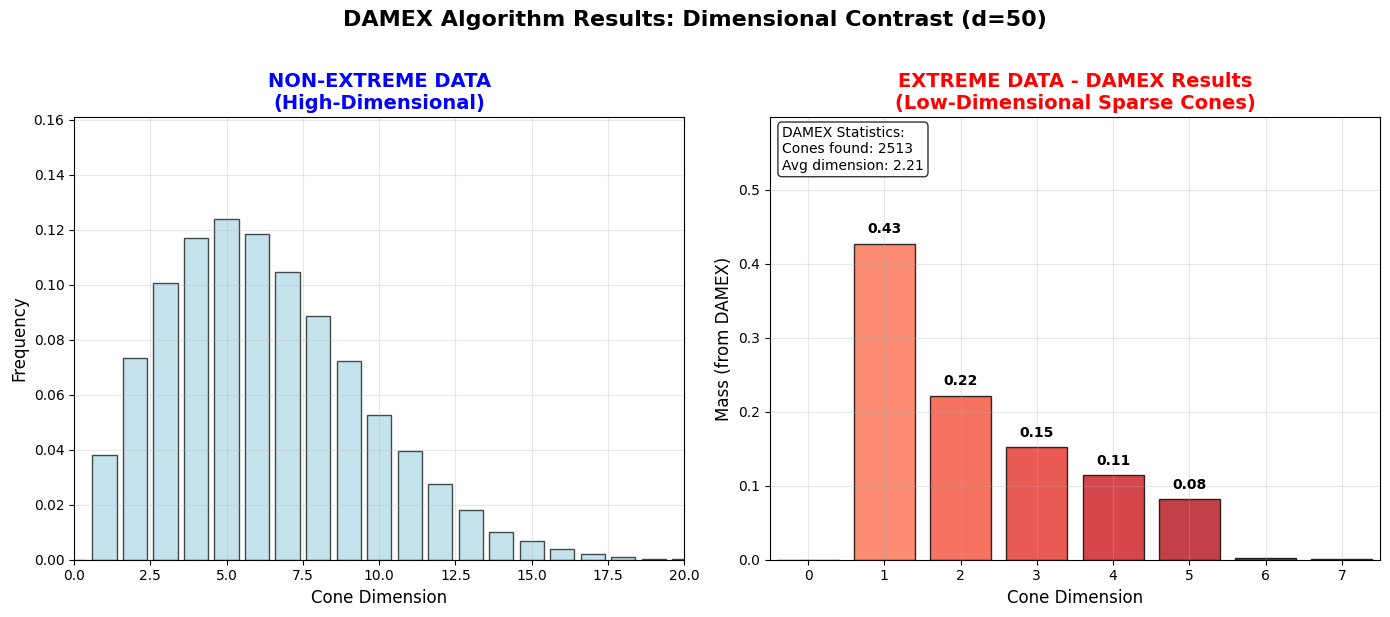
\includegraphics[width=0.7\textwidth]{img/sparsity.png}
    \caption{Distribution of angular mass across cone dimensions for extreme simulated data. 
    The mass is predominantly concentrated on cones of dimension $\leq 5$, confirming the sparsity (Phenomenon I) and low-dimensionality (Phenomenon II) of extremal dependence structures, in alignment with the findings reported in Goix et al. (2017).}
    \label{fig:extreme_sparsity}
\end{figure}



While the non-extreme data spans all 14 dimensions, extreme values cluster in just 5 dimensions, demonstrating the dimensional sparsity characteristic of extremes.
This empirical observation matches the results presented in the original paper, where real-world wave data also showed concentration of extreme mass on a small number of low-dimensional cones. 
Such sparsity enables efficient and interpretable modeling of multivariate extremes, as exploited by the DAMEX algorithm for anomaly detection.

\subsection{DAMEX: Clustering features \cite{jorgensen1997theory, jorgensen1987exponential, cordeiro2021introduction}}

\textbf{Goal:} Find the features that behave the same on the extreme data (data reduction on the extreme values).

Let's say that we have a dataset $(X_i)_{i \in [n]}$ where $X_i \in \mathbb{R}^d$.
In other words we have $n$ data and $d$ features for each data.

A first idea to find the best cluster would be to try out all possible subset $A$ of $[1,d]$.

\textbf{A meaningful cluster is one where the features are dependents.}
To determine if a cluster of features is a good one, the features inside this cluster must behave correlately for all extreme data (on the cone).
Behaving the same for two features $i$ and $j$ can be translated as when $i$ is high $j$ is high and when $j$ is low, $i$ is low. In other word, we can say that if $i$ and $j$ are independent the cluster $A$ having $i$ and $j$ is not a good one however if they are dependent (the behavior of one influence the behavior of the other) $A$ having $i$ and $j$ is a good cluster since with the behavior of one we can have the behavior of the other. 
Hence to test if a cluster is a good one we simply do a dependence test and try to maximize its deviance.

\textbf{Test of dependence to find relevant cluster.}
Let's $A=\{i, j, k\}$, here we only consider the extreme data not the whole dataset but only the extreme dataset.

$H_0$: $P(k \text{ extreme\_data}, i \text{ extreme\_data and } j \text{ extreme\_data}) = P(i \text{ extreme}) P(j \text{ extreme}) P(k \text{ extreme})$

$H_1$: $P(k \text{ extreme\_data}, i \text{ extreme and } j \text{ extreme}) > P(i \text{ extreme}) P(j \text{ extreme}) P(k \text{ extreme})$

\[
\text{DevianceTest}(A) = -2 \times \log\left[ \frac{\text{Likelihood}(\text{Data\_extreme}_{[A]} \mid H_0)}{\text{Likelihood}(\text{Data\_extreme}_{[A]} \mid H_1)} \right]
\]

where $\text{Data\_extreme}_{[A]}$ is the initial dataset where we consider only the extreme data from this dataset and only the features $i \in A$ for this dataset. Hence a high deviance means $\text{Likelihood}(\text{Data\_extreme}_{[A]} \mid H_0) \ll \text{Likelihood}(\text{Data\_extreme}_{[A]} \mid H_1)$ so we get $H_0$ rejected and so the $k$, $i$ and $j$ are dependent, so the cluster is meaningful.
So the dumb approach would be to test all of these subsets and keep only the best clusters $A$. However testing all of these subsets will be computationally costly that's why we use different approach.
We can use CLEF which uses a hierarchical tree method (we will not detail this method here). We can also use DAMEX to preselect our $A$. Instead of testing all subset $A$ of $[1, d]$, we will focus only on the cones, outputs of the DAMEX algorithm. The DAMEX method for clustering is presented in Algorithm~\ref{damex_algorithm} of the section~\ref{sec:damex_algorithm}. To find the best cluster, we use the AIC metric and try to minimize it:

\[
\text{AIC} = \text{Training Deviance} + 2 \times \frac{\# \text{subfaces}}{n_{\text{extremes}}}
\]
where 
\[
\text{Deviance} = \frac{-2}{n_{\text{extremes}}} \times \sum_i \log\left( \sum_j p_j \exp\left(-\text{rate} \times d(X_i, \text{subface}_j)\right) \right)
\]

and here the Training Deviance is computed using cross validation. The lower the training deviance is the better the clustering is since each cluster is close to its subface. Hence minimizing the AIC allows us to find the best compromise between minimizing the variance and don't overparametrize (too many subfaces).

\textbf{Hyperparametrization:}
To get the best feature clustering we have to choose the best epsilon. If epsilon is too high we get too many subfaces (number of clusters) and we might overfit so AIC will be high (because of the numbers of subfaces). If no clusters are found (when $\varepsilon$ is extremely small), then $\text{len(Masses)} = 0$, making the AIC penalty term exactly zero. The deviance would then be computed only for the background model covering all points, but with zero complexity penalty. This explains why $AIC \approx 0$ at minimal epsilon: it essentially reduces to a null model with no subspace structure but pays no penalty for its simplicity. Hence reusing the test done by MLExtreme \cite{mlextreme2023} we can see this shape and an optimal point where the deviance is minimal considering enough points. 

The $\texttt{rate}$ scales $\exp(-\texttt{rate} \times d)$ in the deviance. Larger $\texttt{rate}$ → only very similar subfaces matter. Smaller $\texttt{rate}$ → more tolerance to mismatches. It controls sensitivity in scoring.

The figure~\ref{pseudo_deviance} of the section~\ref{sec:damex_pseudo_deviance} shows four zones, described with $\epsilon$ increasing:
\begin{itemize}
    \item \textbf{Zone 1:} $\epsilon$ is tiny, very few clusters are recognized. Most data points are not assigned to any cluster, leading to near-zero deviance (only perfectly aligned points contribute) and $\#\text{subfaces} \approx 0$. The AIC penalty term $2 \cdot \#\text{subfaces}/\text{number\_extremes}$ becomes negligible, giving $AIC \approx 0$.
    
    \item \textbf{Zone 2:} AIC decreases. The initial peak in AIC occurs when the first non-optimal clusters appear, increasing both deviance and the penalty term. As $\epsilon$ increases, more meaningful clusters are discovered, improving data coverage and reducing deviance faster than the complexity penalty increases.
    
    \item \textbf{Zone 3:} AIC increases. The number of subfaces grows excessively, leading to overfitting. While deviance continues to decrease slightly, the complexity penalty dominates, indicating the model is becoming too specific to the training data.
    
    \item \textbf{Zone 4:} AIC decreases again, demonstrating double descent. With very large $\epsilon$, subfaces become fewer but larger (higher-dimensional), effectively merging into simpler structures. The complexity penalty drops sharply as redundant subfaces collapse, outweighing the slight increase in deviance from less precise modeling.
\end{itemize}

\textbf{Possible improvements:} Consider another AIC which penalizes better the uncovered data without impacting too much the global AIC. 



\subsection{Analysis of Crypto-Crashes}
We applied the DAMEX algorithm (via \texttt{MLExtreme}) to the cryptocurrency returns. The algorithm revealed a highly interpretable dependence structure during market crashes.

\textbf{1. Systemic Risk Identification:}
The algorithm identified a dominant 5-dimensional cone containing cryptocurrencies \texttt{\{BTC, ETH, BNB, SOL, XRP\}}.
\begin{itemize}
    \item \textbf{Observation:} This cone carries the highest probability mass ($\approx 1.0$ in our un-normalized mass output).
    \item \textbf{Interpretation:} This indicates a "Full Dependence" structure among volatile assets. When a major crash occurs, it is rarely isolated; if Bitcoin crashes, the entire altcoin market tends to follow immediately. This confirms that the "diversification" benefit among these assets during extreme events is negligible.
\end{itemize}

\textbf{2. The Stablecoin Decoupling:}
The algorithm identified a distinct, lower-dimensional cone dominated by \texttt{USDT} (Tether).
\begin{itemize}
    \item \textbf{Observation:} \texttt{USDT} extremes often appear in a cone separate from the speculative assets (Mass $\approx 0.73$).
    \item \textbf{Interpretation:} This captures "de-pegging" events or isolated volatility in stablecoins that do not perfectly correlate with the broader market crash. This separation is critical for anomaly detection: a crash in \texttt{USDT} is structurally different from a crash in \texttt{ETH}.
\end{itemize}

\textbf{3. Dimensionality Analysis:}
Table~\ref{tab:crypto_results} summarizes the mass distribution. We observe "Phenomenon II" (low dimensionality) only partially: while specific subsets exist (e.g., \texttt{SOL + USDT}), the dominance of the full-dimensional cone suggests that the crypto market is highly integrated, unlike the wave data presented in the original paper where physical constraints enforce sparsity.

\begin{table}[h]
    \centering
    \begin{tabular}{llc}
        \toprule
        \textbf{Dimension} & \textbf{Cone (Assets)} & \textbf{Relative Mass} \\
        \midrule
        5 (Cryptocurrencies) & BTC + ETH + BNB + SOL + XRP & 1.0007 \\
        1 & USDT & 0.7278 \\
        6 (Full) & BTC + ETH + BNB + SOL + XRP + USDT & 0.6368 \\
        4 & BNB + BTC + ETH + XRP & 0.3639 \\
        2 & SOL + USDT & 0.1819 \\
        \bottomrule
    \end{tabular}
    \caption{Dominant dependence cones identified by DAMEX in the Crypto dataset. The market exhibits a split structure: a highly dependent speculative block and a decoupled stablecoin component.}
    \label{tab:crypto_results}
\end{table}


\section{Conclusion and Discussion}
The paper successfully demonstrates that incorporating multivariate Extreme Value Theory into anomaly detection yields significant improvements for tail events. By explicitly modeling the sparse dependence structure of extremes using $\epsilon$-thickened cones, DAMEX overcomes the curse of dimensionality that plagues standard kernel-based or nearest-neighbor methods in high-dimensional spaces.

However, the method relies on sensitive hyperparameters, specifically the threshold $k$ (bias-variance trade-off) and the tolerance $\epsilon$. While the theoretical bounds provided in the paper offer a framework for understanding these trade-offs, practical selection remains heuristic. Future work could focus on adaptive selection of $\epsilon$ or supervised optimization of these parameters when labels are available.

\bibliographystyle{plainnat}
\bibliography{bibliography}

\newpage
\appendix
\section{Appendix: DAMEX Algorithm}\label{sec:damex_algorithm}
\begin{algorithm}
\caption{DAMEX $\epsilon$ Selection Pipeline (Visual Sketch)}
\label{damex_algorithm}
\begin{algorithmic}[1]
\Procedure{SelectBestEpsilon}{}
    \State $\mathcal{E} \gets \{\epsilon_1, \epsilon_2, \dots, \epsilon_m\}$
    
    \For{$\epsilon \in \mathcal{E}$}
        \State $\triangleright$ \textbf{DAMEX($\epsilon$)} finds candidates $\mathcal{A}_\epsilon = \{A_1, A_2, \dots\}$
        
        \State $\mathcal{S}_\epsilon \gets \emptyset$
        \For{$A \in \mathcal{A}_\epsilon$}
            \If{$\text{DevianceTest}(A)$ is significant}
                \State $\mathcal{S}_\epsilon \gets \mathcal{S}_\epsilon \cup \{A\}$
            \EndIf
        \EndFor
        
        \State $\triangleright$ \textbf{Compute training deviance from $\mathcal{S}_\epsilon$}
        \State $\text{TD}_\epsilon \gets \text{TrainingDeviance}(\mathcal{S}_\epsilon)$
        
        \State $\triangleright$ \textbf{Compute AIC}
        \State $\text{AIC}_\epsilon \gets \text{TD}_\epsilon + 2 \cdot \dfrac{|\mathcal{S}_\epsilon|}{n}$
    \EndFor
    
    \State $\triangleright$ \textbf{Select $\epsilon^*$ with minimum AIC}
    \State $\epsilon^* \gets \arg\min_{\epsilon \in \mathcal{E}} \text{AIC}_\epsilon$
    
    \State \Return $\epsilon^*$
\EndProcedure
\end{algorithmic}
\end{algorithm}


\section{Appendix: DAMEX clustering pseudo-deviance}\label{sec:damex_pseudo_deviance}
\begin{figure}[h]
    \centering
    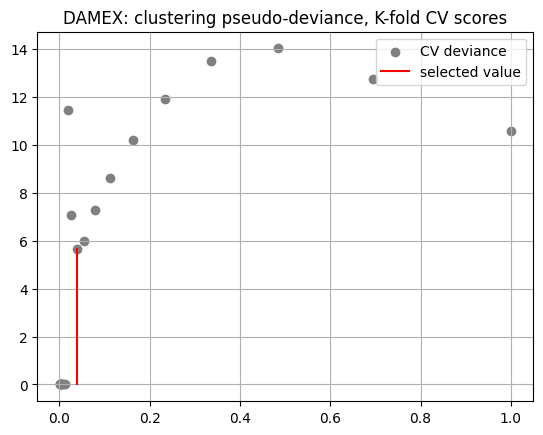
\includegraphics[width=0.8\textwidth]{img/AIC_eps.png}
    \caption{Relationship between epsilon and AIC/deviance metrics}
    \label{pseudo_deviance}
\end{figure}

\end{document}